% !TeX program = pdflatex
% Generic, organization-agnostic architecture discovery guide.
% Compile: latexmk -pdf -interaction=nonstopmode -halt-on-error GitHub_Actions_Architecture_Discovery_Guide.tex
\documentclass[11pt,letterpaper]{article}
\usepackage[T1]{fontenc}
\usepackage[utf8]{inputenc}
\usepackage{lmodern}
\usepackage{microtype}
\usepackage[margin=0.93in,headheight=22pt,headsep=22pt,footskip=30pt]{geometry}
\usepackage{graphicx}
\usepackage{booktabs,tabularx,longtable,array,multirow}
\usepackage{enumitem}
\usepackage{titlesec}
\usepackage{fancyhdr}
\usepackage{lastpage}
\usepackage{xcolor}
\usepackage[most]{tcolorbox}
\usepackage{tikz}
\usetikzlibrary{arrows.meta,positioning,fit,shapes.geometric,calc}
\usepackage{listings}
\usepackage{caption}
\usepackage{hyperref}
\usepackage{xurl}
\usepackage{float}
\usepackage{needspace}
\usepackage{parskip}
\usepackage{etoolbox}
\usepackage{ragged2e}
\usepackage{amssymb}

\definecolor{Navy}{HTML}{142B43}
\definecolor{Deep}{HTML}{0C2034}
\definecolor{Teal}{HTML}{087F78}
\definecolor{Sea}{HTML}{DDF3EF}
\definecolor{BlueGray}{HTML}{51677D}
\definecolor{Pale}{HTML}{F2F6F9}
\definecolor{Rule}{HTML}{D9E2E9}
\definecolor{Amber}{HTML}{A66A16}
\definecolor{AmberPale}{HTML}{FFF5E7}
\definecolor{CodeBg}{HTML}{F4F7FA}

\hypersetup{colorlinks=true,linkcolor=Navy,urlcolor=Teal,citecolor=Teal,pdfauthor={Architecture Engineering Reference},pdftitle={GitHub Actions Architecture Discovery at Enterprise Scale},pdfsubject={Evidence-driven repository, CI, component, and dependency discovery}}
\setlength{\parindent}{0pt}
\setlength{\parskip}{6.2pt}
\setlist[itemize]{leftmargin=*,itemsep=2pt,topsep=3pt}
\setlist[enumerate]{leftmargin=*,itemsep=3pt,topsep=3pt}
\setlength{\emergencystretch}{2em}
\renewcommand{\arraystretch}{1.23}
\captionsetup{font=small,labelfont={bf,color=Navy},textfont={color=BlueGray}}
\titleformat{\section}{\Large\bfseries\color{Navy}}{\thesection}{0.8em}{}[\vspace{-1pt}{\color{Teal}\titlerule[1.2pt]}]
\titleformat{\subsection}{\large\bfseries\color{Navy}}{\thesubsection}{0.75em}{}
\titleformat{\subsubsection}{\normalsize\bfseries\color{Teal}}{\thesubsubsection}{0.6em}{}
\titlespacing*{\section}{0pt}{23pt}{12pt}
\titlespacing*{\subsection}{0pt}{15pt}{7pt}
\titlespacing*{\subsubsection}{0pt}{11pt}{4pt}
\pagestyle{fancy}
\fancyhf{}
\fancyhead[L]{\footnotesize\color{BlueGray}\sffamily ARCHITECTURE ENGINEERING / TECHNICAL GUIDE}
\fancyhead[R]{\footnotesize\color{Teal}\sffamily GITHUB ACTIONS}
\fancyfoot[L]{\footnotesize\color{BlueGray} Reference edition \textbullet\ October 2026}
\fancyfoot[R]{\footnotesize\color{BlueGray} \thepage\ / \pageref{LastPage}}
\renewcommand{\headrulewidth}{0.5pt}
\renewcommand{\headrule}{\hbox to\headwidth{\color{Rule}\leaders\hrule height \headrulewidth\hfill}}
\renewcommand{\footrulewidth}{0pt}
\fancypagestyle{plain}{\fancyhf{}\fancyfoot[R]{\footnotesize\color{BlueGray}\thepage\ / \pageref{LastPage}}\renewcommand{\headrulewidth}{0pt}}

\newtcolorbox{keypoint}[1][]{enhanced,breakable,colback=Sea,colframe=Teal,boxrule=0.65pt,arc=2mm,left=12pt,right=12pt,top=9pt,bottom=9pt,before skip=9pt,after skip=10pt,#1}
\newtcolorbox{cautionbox}[1][]{enhanced,breakable,colback=AmberPale,colframe=Amber,boxrule=0.6pt,arc=2mm,left=12pt,right=12pt,top=9pt,bottom=9pt,before skip=9pt,after skip=10pt,#1}
\newcommand{\eyebrow}[1]{{\sffamily\bfseries\small\color{Teal}\MakeUppercase{#1}}}
\newcommand{\term}[1]{\textbf{\color{Navy}#1}}
\newcommand{\code}[1]{{\small\ttfamily\detokenize{#1}}}
\newcommand{\source}[1]{\textsuperscript{\hyperref[ref:#1]{[#1]}}}
\newcolumntype{Y}{>{\RaggedRight\arraybackslash}X}
\newcolumntype{P}[1]{>{\RaggedRight\arraybackslash}p{#1}}
\lstdefinestyle{guide}{basicstyle=\footnotesize\ttfamily,backgroundcolor=\color{CodeBg},frame=single,rulecolor=\color{Rule},framesep=9pt,breaklines=true,breakatwhitespace=false,showstringspaces=false,tabsize=2,keywordstyle=\color{Teal}\bfseries,commentstyle=\color{BlueGray},stringstyle=\color{Navy},columns=fullflexible,keepspaces=true,upquote=true,aboveskip=9pt,belowskip=9pt}
\lstset{style=guide}

\begin{document}
\thispagestyle{empty}
\begin{tikzpicture}[remember picture,overlay]
 \fill[Deep] (current page.north west) rectangle ([yshift=-4.13in]current page.north east);
 \fill[Teal] ([xshift=0.93in,yshift=-3.71in]current page.north west) rectangle ([xshift=6.15in,yshift=-3.64in]current page.north west);
 \draw[white,opacity=0.13,line width=1.2pt] ([xshift=5.7in,yshift=-0.7in]current page.north west) circle (1.38in);
 \draw[white,opacity=0.1,line width=1.2pt] ([xshift=6.9in,yshift=-2.8in]current page.north west) circle (1.6in);
\end{tikzpicture}
\vspace*{0.86in}
{\color{white}\sffamily\fontsize{12}{16}\selectfont TECHNICAL ARCHITECTURE REFERENCE}\par
\vspace{0.28in}
{\color{white}\sffamily\bfseries\fontsize{28}{34}\selectfont GitHub Actions\\[3pt] Architecture Discovery\\[3pt] at Enterprise Scale}\par
\vspace{0.26in}
{\color{white}\fontsize{13}{19}\selectfont An evidence-driven method for mapping repositories,\\ workflows, components, build artifacts, and dependencies}\par
\vspace{1.36in}
\eyebrow{Purpose}\par
\vspace{7pt}
{\Large\bfseries\color{Navy} From CI configuration to a defensible\\ application architecture catalog}\par
\vspace{14pt}
{\color{BlueGray}Designed for large GitHub organizations, including portfolios with thousands of repositories and heterogeneous monorepos. This guide is independent of any particular organization or source-code estate.}\par
\vfill
\begin{tabularx}{\linewidth}{@{}P{1.15in}Y@{}}
\color{BlueGray}\textbf{Audience} & Platform engineering, enterprise architecture, AppSec, DevOps, application ownership teams \\
\color{BlueGray}\textbf{Status} & Reference architecture and implementation methodology \\
\color{BlueGray}\textbf{Edition} & October 2026 \quad | \quad Version 1.0 \\
\end{tabularx}
\newpage

\section*{Executive summary}
A large GitHub estate cannot be understood reliably by treating every repository as an application or by reading every source file. GitHub Actions workflow definitions provide a scalable \emph{starting point}: they expose job orchestration, reusable workflow calls, build commands, artifact publication hints, deployment targets and path-scoped automation. But workflow YAML is not a complete representation of runtime architecture.

This guide presents a read-only discovery pipeline that inventories GitHub repositories, parses CI configurations, identifies candidate components in monorepos, produces an evidence-backed graph, and progressively correlates the results with deployment and runtime sources. The primary outcome is an \term{architecture inventory that communicates what is known, how it was learned, and what remains unverified}.

\begin{keypoint}
\textbf{Governing principle.} CI configuration is a high-value architectural signal, \emph{not} an infallible source of truth. Treat explicit configuration edges, parser-derived inferences, and independently verified runtime relationships as distinct classes of evidence. Never promote a build or deployment command into a proven runtime dependency without corroboration.
\end{keypoint}

\begin{tabularx}{\linewidth}{@{}P{1.7in}Y@{}}
\toprule
\textbf{Design objective} & \textbf{Expected property} \\
\midrule
Scale & Inventory thousands of repositories without routine full clones. \\
Traceability & Each discovered relationship links back to a file path, revision, and extraction rule. \\
Monorepo fidelity & Count applications and deployable components separately from repositories. \\
Operational safety & Read-only credentials, bounded API demand, and no evaluation of untrusted scripts. \\
Reproducibility & Incremental snapshots, stable entity identifiers, and explicit parser versions. \\
Trustworthiness & Coverage, confidence, missing evidence, and uncertainty are first-class outputs. \\
\bottomrule
\end{tabularx}

\vspace{3pt}
\tableofcontents

\section{Scope, terminology, and architectural boundaries}
\subsection{The unit-of-analysis problem}
A \term{repository} is a version-controlled collection of files. A \term{workflow} is a YAML-defined automation that runs one or more jobs. A \term{component} is an independently identifiable package, module, library, or service candidate. An \term{application} is a logical product or capability that may span multiple deployable components and repositories. A \term{deployment} is a release of a concrete artifact to an identified target. These concepts must not be collapsed into a one-to-one mapping.

A single monorepo might host a web frontend, three services, two reusable libraries, and multiple independent delivery workflows. Conversely, a single business application may comprise separate API, web, infrastructure, and operational repositories.

\subsection{In scope and out of scope}
\begin{tabularx}{\linewidth}{@{}P{1.55in}Y@{}}
\toprule
\textbf{In scope} & \textbf{Requires independent enrichment} \\
\midrule
Repositories and revisions & Actual ownership and accountable service teams \\
Workflow triggers, jobs, and job dependencies & Verified runtime call graphs and production traffic \\
Reusable workflows and external actions & Executed behavior of arbitrary third-party actions \\
Workspace and package declarations & Full language-level dependency resolution \\
Build contexts, image destinations, artifact hints & Artifact deployment success and live inventory \\
Deployment environments referenced in YAML & Actual infrastructure resources and service health \\
\bottomrule
\end{tabularx}

\subsection{Operating assumptions}
The reference implementation assumes GitHub Actions, organization or enterprise-level authorized read access, a mix of standard repositories and monorepos, and primarily \emph{static analysis of a pinned revision}. Workflow-run history, artifact registries, IaC, deployment APIs, and runtime telemetry are optional enrichment tiers. Multi-organization deployments may require separate installation credentials and access partitions.

\section{Reference architecture}
The architecture separates collection, parsing, correlation, storage, and presentation so that ambiguous source evidence does not contaminate verified relationships.

\begin{figure}[H]
\centering
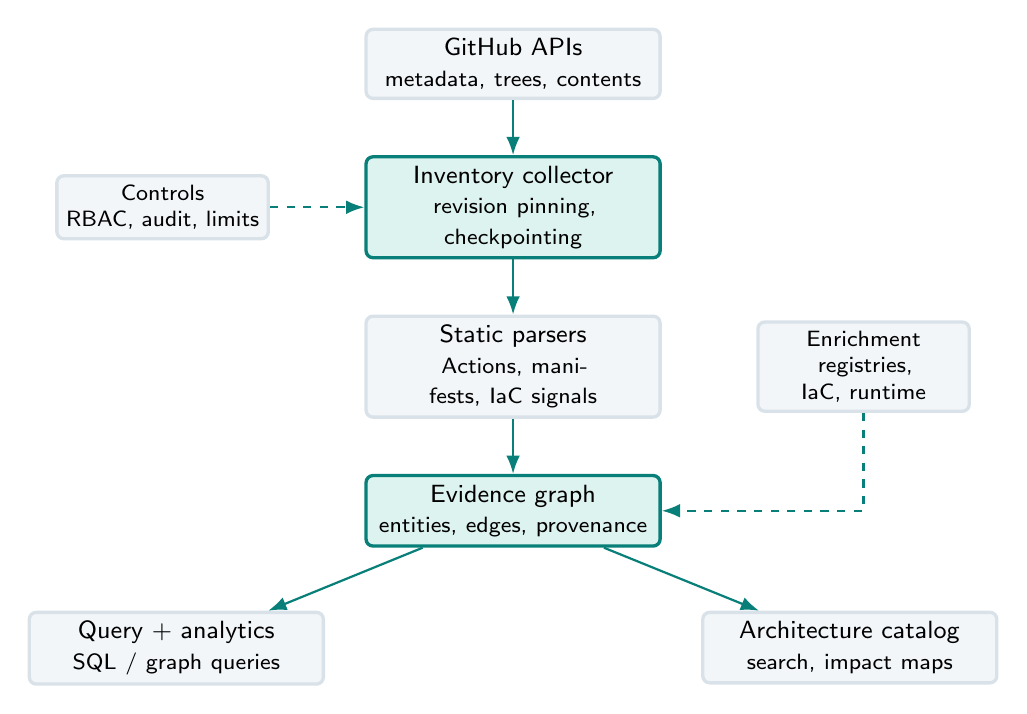
\begin{tikzpicture}[
  node distance=7mm,
  x=1cm,y=1cm,
  block/.style={draw=Rule,rounded corners=2.5pt,fill=Pale,very thick,minimum height=0.82cm,align=center,text width=3.5cm,font=\small\sffamily},
  strong/.style={block,draw=Teal,fill=Sea},
  flow/.style={-Latex,thick,color=Teal},
  side/.style={block,text width=2.45cm,minimum height=0.65cm,font=\footnotesize\sffamily}
]
\node[block] (api) {GitHub APIs\\\footnotesize metadata, trees, contents};
\node[strong,below=of api] (collect) {Inventory collector\\\footnotesize revision pinning, checkpointing};
\node[block,below=of collect] (parse) {Static parsers\\\footnotesize Actions, manifests, IaC signals};
\node[strong,below=of parse] (graph) {Evidence graph\\\footnotesize entities, edges, provenance};
\node[block,below left=8mm and 5mm of graph] (query) {Query + analytics\\\footnotesize SQL / graph queries};
\node[block,below right=8mm and 5mm of graph] (catalog) {Architecture catalog\\\footnotesize search, impact maps};
\node[side,right=12mm of parse] (runtime) {Enrichment\\\footnotesize registries, IaC, runtime};
\node[side,left=12mm of collect] (control) {Controls\\\footnotesize RBAC, audit, limits};
\draw[flow] (api) -- (collect);
\draw[flow] (collect) -- (parse);
\draw[flow] (parse) -- (graph);
\draw[flow] (graph) -- (query);
\draw[flow] (graph) -- (catalog);
\draw[flow,dashed] (runtime) |- (graph.east);
\draw[flow,dashed] (control) -- (collect);
\end{tikzpicture}
\caption{Logical pipeline. Solid lines represent the baseline inventory flow; dashed lines indicate cross-cutting governance or optional evidence enrichment.}
\label{fig:logical}
\end{figure}

\subsection{Processing stages}
\begin{enumerate}
\item \term{Discover:} enumerate authorized organizations and repositories, capturing IDs, lifecycle state, default branch, topics, timestamps, and visibility.
\item \term{Pin:} resolve each repository's selected branch to a commit SHA; use that SHA for content retrieval and provenance.
\item \term{Inspect:} locate workflows, workspace manifests, package descriptors, Dockerfiles, and relevant IaC without a full clone.
\item \term{Parse:} convert YAML and manifest structures to typed normalized facts; preserve unresolved expressions instead of guessing.
\item \term{Correlate:} join job, component, artifact, project, and deployment hints using explicit rules and evidence classes.
\item \term{Publish:} store graph nodes and edges, validation warnings, inventory coverage, and queryable snapshots.
\end{enumerate}

\section{Discovery inputs and extraction rules}
\subsection{Source files to prioritize}
\begin{longtable}{@{}P{2.4in}P{2.25in}P{1.65in}@{}}
\toprule
\textbf{Source} & \textbf{Primary signal} & \textbf{Interpretation} \\
\midrule
\endhead
\code{.github/workflows/*.yml}, \code{*.yaml} & Events, jobs, build and publish steps, environments & Strong CI topology evidence \\
\code{action.yml}, \code{action.yaml} & Composite or local action behavior & Action reuse; indirect execution \\
\code{Dockerfile}, \code{docker-bake.hcl} & Build context, stages, target images & Buildable artifact candidate \\
\code{pom.xml}, \code{build.gradle(.kts)} & Java build modules and artifacts & Package/module identity \\
\code{package.json}, lockfiles & Package identity and scripts & JS/TS package candidate \\
\code{pnpm-workspace.yaml}, \code{nx.json}, \code{turbo.json} & Workspaces and task graph hints & Monorepo candidate \\
\code{pyproject.toml}, \code{uv.lock} & Python project/package metadata & Package identity \\
\code{go.mod}, \code{Cargo.toml} & Go/Rust module/crate metadata & Component identity \\
\code{*.tf}, Helm charts, Kustomize & Infrastructure/deployment definitions & Correlation inputs only \\
\bottomrule
\end{longtable}

GitHub Actions workflows are typically defined in \code{.github/workflows/}, with their triggers and jobs represented in YAML.\source{1} Query only relevant file paths and trees initially; fall back to targeted sub-tree retrieval when the recursive tree result is truncated.\source{2}

\subsection{Key workflow fields}
Extract trigger and job definitions (\code{on}, \code{jobs.<id>}, \code{needs}, and \code{runs-on}); step actions and commands (\code{steps[*].uses}, \code{steps[*].run}); reusable workflow calls (\code{jobs.<id>.uses}); and matrix, environment, and working-directory metadata. Normalize explicit calls and file references separately from free-form command text.

\begin{lstlisting}[language={},caption={Illustrative workflow; all names are placeholders.}]
name: build-and-release
on:
  push:
    paths:
      - 'services/billing/**'
  workflow_dispatch:
jobs:
  test:
    runs-on: ubuntu-latest
    defaults:
      run:
        working-directory: services/billing
    steps:
      - uses: actions/checkout@v4
      - run: ./mvnw test
  publish:
    needs: test
    uses: example-org/ci/.github/workflows/publish.yml@v2
    with:
      image-name: billing-api
\end{lstlisting}

\begin{cautionbox}
\textbf{Parser correctness.} YAML 1.1 loaders can interpret the unquoted key \code{on} as a boolean. Select a parser or configuration that preserves GitHub Actions keys as intended. Do not execute \code{run} content, resolve secrets, or evaluate shell substitutions during static discovery. Reusable workflow calls reside at \code{jobs.<job>.uses}, whereas ordinary actions are typically referenced in \code{steps[*].uses}.\source{3}
\end{cautionbox}

\subsection{Relationship semantics}
\begin{tabularx}{\linewidth}{@{}P{2.35in}Y@{}}
\toprule
\textbf{Edge type} & \textbf{Evidence requirement} \\
\midrule
\code{REPOSITORY_HAS_WORKFLOW} & Workflow file observed at a pinned commit. \\
\code{WORKFLOW_HAS_JOB} & Job key exists in parsed workflow. \\
\code{JOB_NEEDS_JOB} & Explicit \code{needs} reference within a workflow. \\
\code{JOB_CALLS_WORKFLOW} & Literal \code{jobs.<id>.uses} reusable workflow target. \\
\code{JOB_USES_ACTION} & Literal \code{steps[*].uses} target. \\
\code{REPOSITORY_HAS_COMPONENT} & Identifiable package or workspace manifest. \\
\code{JOB_BUILDS_COMPONENT} & Explicit target/path match, with inference flagged. \\
\code{JOB_PUBLISHES_ARTIFACT} & Registry/package destination derived from an explicit field or command; distinguish declaration from successful publish. \\
\code{ARTIFACT_DEPLOYED_TO} & Only after corroborated deployment evidence, not on static YAML alone. \\
\bottomrule
\end{tabularx}

GitHub workflow path filters narrow when automation runs; they do not alone prove the ownership or dependency boundary of the matching component. Both branch and path filters may apply together.\source{4}

\section{Monorepo discovery and component resolution}
\subsection{Component inventory over repository count}
Store repository, component, application, and artifact identifiers separately. Begin with workspace declarations, then resolve concrete workspace paths only when file-tree evidence is available. Use manifest package names as candidate identities, but prevent collisions with a namespaced key that includes repository ID and relative location.

\begin{keypoint}
\textbf{Recommended identifier.} \code{component:<repository-id>:<relative-path>} is stable for a snapshot; maintain a separate durable component UUID and path-history mapping when packages move or repositories are renamed.
\end{keypoint}

\subsection{Discovery process}
\begin{enumerate}
\item Detect package managers, workspace declaration files, and root-level project configuration.
\item Expand package globs against the pinned tree, respecting exclusion patterns and tooling-specific semantics.
\item Record package/module identities, explicit manifest dependencies, task definitions, and paths.
\item Associate jobs with candidate components using path filters, job working directories, Docker build contexts, and explicit build targets.
\item Treat ambiguous broad patterns and matrix-generated paths as unresolved until expanded or corroborated.
\end{enumerate}

\subsection{Important exceptions}
\begin{itemize}
\item \term{Polyglot monorepos:} a single repository may contain independent Maven, pnpm, Python, and Go build systems.
\item \term{Dynamic build logic:} shell-generated target names, scripts, and composite actions limit static visibility.
\item \term{Unpublished packages:} a workspace module may be an internal utility, not a deployable service.
\item \term{Sparse and nested checkouts:} checkout steps can pull another repository or selected paths, changing the effective build inputs.
\item \term{Reusable workflow indirection:} inspect the referenced workflow at its declared revision, preserving access limitations and nested calls.
\end{itemize}

\section{Normalized evidence and graph model}
\subsection{Entity schema}
The model should support the entities \term{Organization}, \term{Repository}, \term{Revision}, \term{Workflow}, \term{Job}, \term{Action}, \term{Component}, \term{Artifact}, \term{Environment}, and \term{Deployment}. Application and Team become authoritative only when matched to approved catalog or ownership records.

\begin{table}[H]
\centering\small
\begin{tabularx}{\linewidth}{@{}P{1.4in}Y@{}}
\toprule
\textbf{Attribute} & \textbf{Meaning} \\
\midrule
\code{source_uri} & URL for the GitHub file or corresponding authoritative record. \\
\code{source_path} & Repository-relative file path or external record key. \\
\code{commit_sha} & Exact inspected revision for file-derived observations. \\
\code{extraction_rule} & Versioned rule name and parser version. \\
\code{evidence_class} & \code{observed}, \code{inferred}, or \code{verified}. \\
\code{confidence} & Numeric or categorical quality assessment; not a substitute for evidence class. \\
\code{collected_at} & Snapshot collection timestamp, UTC. \\
\code{status} & \code{current}, \code{stale}, \code{unresolved}, \code{denied}, or \code{error}. \\
\bottomrule
\end{tabularx}
\caption{Minimum lineage and trust metadata for graph relationships.}
\end{table}

\subsection{Evidence classes and promotion rules}
\begin{enumerate}[label=\textbf{E\arabic*.}]
\item \term{Observed configuration:} direct parse of a workflow key, manifest field, or immutable source path.
\item \term{Inferred relationship:} parser rule connects build context, artifact, or directory patterns to a candidate component; record the rule and ambiguity.
\item \term{Externally verified:} corroborated by a deployment record, registry digest, service catalog, cloud resource inventory, or approved owner assertion.
\end{enumerate}

Inferences should not be described as confirmed architecture. Keep competing hypotheses and negative results. A missing workflow might indicate no workflow, an inaccessible repository, a non-default branch, or an interrupted scan.

\subsection{Sample graph queries}
\begin{lstlisting}[language=SQL,caption={Investigate reusable workflow dependencies in a normalized SQL view.}]
SELECT source_id, target_id, source_uri, evidence_class
FROM architecture_edges
WHERE edge_type = 'JOB_CALLS_WORKFLOW'
  AND status = 'current'
ORDER BY target_id, source_id;
\end{lstlisting}

\begin{lstlisting}[language={},caption={Cypher example: candidate components associated with build jobs.}]
MATCH (r:Repository)-[:REPOSITORY_HAS_COMPONENT]->(c:Component)
MATCH (j:Job)-[e:JOB_BUILDS_COMPONENT]->(c)
WHERE e.evidence_class IN ['observed', 'inferred']
RETURN r.name, c.name, j.name, e.evidence_class
ORDER BY r.name, c.name;
\end{lstlisting}

\section{Collection implementation}
\subsection{Authentication and API access}
For scalable read-only collection, prefer a GitHub App installation scoped to authorized repositories. Request only permissions required by the selected endpoints; repository metadata and contents read are typical baseline needs, while retrieving workflow execution history requires additional API access. Review permissions against the endpoint reference rather than assuming a universal token profile.\source{5}\source{6}

\subsection{API and data retrieval strategy}
\begin{enumerate}
\item Enumerate permitted repositories with pagination and record the source organization/installation.
\item Resolve default branch or configured branch to a commit SHA.
\item Retrieve a repository tree for candidate workflow and manifest paths.
\item If Git Trees reports \code{truncated=true}, traverse subtrees non-recursively until coverage is explicit.\source{2}
\item Fetch only selected files, use content hashes for change detection, and cache parsed facts by immutable SHA and parser version.
\item Persist checkpoints and statuses before moving to the next work queue partition.
\end{enumerate}

\subsection{Illustrative command-line contract}
The following shows how an optional inventory CLI \emph{could} be invoked. The flags describe an implementation interface, not native GitHub CLI commands.

\begin{lstlisting}[language=bash,caption={Example wrapper invocation with generic organization names.}]
python inventory.py \
  --org example-org \
  --max-repos 50 \
  --output-dir ./pilot-inventory

python inventory.py \
  --org example-org \
  --output-dir ./enterprise-inventory
\end{lstlisting}

A production collector should expose limits, retry policy, cache directory, revision mode, access-status reporting, and parser version in its manifest. It must distinguish a full portfolio snapshot from an intentionally bounded pilot.

\subsection{Canonical outputs}
\begin{tabularx}{\linewidth}{@{}P{1.75in}Y@{}}
\toprule
\textbf{Output} & \textbf{Contents} \\
\midrule
\code{repositories.csv} & Repository identifiers, selected branch/commit, lifecycle metadata, coverage state. \\
\code{workflows.csv} & Workflow IDs, triggers, paths, revision, parse status. \\
\code{jobs.csv} & Job identities, runners, dependencies, working directories, matrix declarations. \\
\code{components.csv} & Candidate component identity, manifest origin, workspace paths. \\
\code{relationships.csv} & Typed edges, source provenance, evidence class, extraction rule. \\
\code{warnings.csv} & Rate limits, API denial, truncated trees, malformed or oversize files. \\
\code{summary.json} & Scan totals, parser version, completeness, timestamps, errors. \\
\bottomrule
\end{tabularx}

\section{Scale, reliability, and operational design}
\subsection{Bounded concurrency and rate limiting}
The GitHub REST API has primary and secondary rate limits. A resilient scanner must honor \code{Retry-After} and primary reset headers, back off on secondary throttling, and avoid high fan-out bursts. Installation-based GitHub App limits vary by plan and installation characteristics; do not hardcode a universal request allowance.\source{7}

\begin{enumerate}
\item Use a queue with bounded per-installation concurrency and centralized request accounting.
\item Apply conditional requests where supported, immutable-content caching, and low-cost tree scans before file downloads.
\item Persist progress per repository and branch so interrupted runs can resume without duplicated parsing.
\item Separate \code{not found}, \code{access denied}, \code{rate limited}, \code{parse failed}, and \code{no evidence} statuses.
\item Use periodic baseline scans and event-driven or scheduled incremental updates.
\end{enumerate}

\subsection{Capacity planning model}
Let \(R\) denote repositories, \(q\) average metadata/tree requests per repository, \(f\) average selected file requests, \(h\) the cache-hit fraction, and \(k\) additional requests due to retries, access checks, and overflow handling. A rough API demand estimate is:
\[
  Q \approx R\bigl(q+f(1-h)\bigr)+k.
\]
For an illustrative 5,000-repository estate with \(q=2\), \(f=8\), \(h=0.75\), and \(k=0\), \(Q\approx20{,}000\) requests per scan. This is an engineering sizing example, \emph{not} a prediction of elapsed time or a GitHub API quota.

\subsection{Completeness metrics}
Track repository access coverage, tree coverage, parse success, identified workflow coverage, resolved workspace coverage, and verified application correlation separately. Sample formulas are:
\[
  C_{\mathrm{repos}}=\frac{\text{repositories successfully inspected}}{\text{repositories in authorized scope}},
  \qquad
  C_{\mathrm{parse}}=\frac{\text{files parsed}}{\text{files selected for parsing}}.
\]
Report denominator exclusions and unknown scope clearly. A high workflow parse rate does not establish high application discovery accuracy.

\section{Security, privacy, and governance}
\begin{itemize}
\item \term{Least privilege:} read-only GitHub App access, narrowly scoped installations, short-lived installation tokens, and regular permission reviews.
\item \term{No untrusted execution:} do not run discovered shell commands, dependency installation hooks, third-party actions, or arbitrary build scripts in the crawler.
\item \term{Credential hygiene:} do not emit secret values, authorization headers, or raw private workflow payloads into logs and analytics exports.
\item \term{Data classification:} architecture graphs can disclose internal names, deployment endpoints, security posture, and cross-system relationships. Apply portfolio-appropriate access control and retention.
\item \term{Provenance:} retain hashes, parser versions, source links, collection timestamps, access failures, and human overrides.
\item \term{Change control:} keep repository metadata and workflow modification functions outside the discovery application's permissions. Treat automated topic tagging or repository edits as separate, approved workflows.
\item \term{Approval boundaries:} deployment/run-history enrichment must not be treated as authorization to change environments or release software.
\end{itemize}

\begin{cautionbox}
\textbf{Sensitive inference risk.} CI configurations may reference internal infrastructure, security tooling, registry locations, and privileged environments. A read-only scanner can still create a sensitive aggregation of metadata. Protect the resulting catalog as an architectural intelligence asset.
\end{cautionbox}

\section{Validation and acceptance criteria}
\subsection{Recommended validation approach}
Start with a stratified sample of small single-service repositories, large monorepos, private and archived repositories, reusable-workflow callers, multiple languages, and known CI edge cases. Compare extracted facts with human-reviewed workflow graphs and accepted service ownership records.

\begin{tabularx}{\linewidth}{@{}P{1.9in}Y@{}}
\toprule
\textbf{Control} & \textbf{Acceptance condition} \\
\midrule
Determinism & Same pinned revision and parser version produce equivalent normalized facts. \\
Safety & Collection runs without write scopes, arbitrary command execution, or leaked tokens. \\
Lineage & Every non-manual edge resolves to a rule, path/record, and revision or external record ID. \\
Monorepo handling & Components are not counted solely by repository name; ambiguous globs are flagged. \\
Error classification & Inaccessible, missing, truncated, and malformed inputs are differentiated. \\
Idempotency & Repeated scans do not duplicate nodes or relationships. \\
Accuracy & Precision/recall measured against a reviewed benchmark before architecture assertions are published. \\
\bottomrule
\end{tabularx}

\subsection{Validation measures}
For manually reviewed sample sets, calculate precision \(P=TP/(TP+FP)\) and recall \(R=TP/(TP+FN)\) separately for explicit CI edges, inferred component matches, and deployment correlations. These are different classification tasks and should not be combined into a single opaque score.

\section{Implementation roadmap}
\begin{longtable}{@{}P{0.75in}P{2.05in}P{3.25in}@{}}
\toprule
\textbf{Phase} & \textbf{Deliverable} & \textbf{Exit criteria} \\
\midrule
\endhead
0 & Scope and control plane & Authorized repository boundary, permission matrix, vocabulary, data retention, and baseline coverage denominator. \\
1 & Read-only pilot collector & Pinned repositories, workflows, jobs, warnings, resumable scans; reviewed representative sample. \\
2 & Monorepo component discovery & Workspace expansion, manifest identities, component-to-job hints, ambiguity reporting. \\
3 & Graph and evidence model & Durable node IDs, typed edges, provenance, SQL/graph queries, repeatable snapshots. \\
4 & Artifact and environment correlation & Registry packages, release metadata, IaC resources, deployment records, provenance links. \\
5 & Governance and catalog views & Searchable portfolio, ownership reconciliation, confidence labels, access control, drift detection. \\
\bottomrule
\end{longtable}

\subsection{Minimum viable deliverable}
The first production-worthy milestone should answer these questions with traceable evidence: \emph{What repositories were scanned? Which workflows and jobs exist? Which jobs depend on others? Which repositories call shared workflows? Which components are declared by monorepos? Which associations are unresolved?} That milestone should \emph{not} claim to identify every production service dependency.

\subsection{Architecture decision checklist}
Before promoting the collector into a standing platform capability, record decisions on the GitHub App access model, storage engine (relational vs. graph), identifier design, static parser scope, update cadence, retention, confidence policy, handling of inaccessible repositories, and runtime enrichment ownership. These decisions can be tracked as versioned Architecture Decision Records.

\section{Reference operating procedure}
\begin{enumerate}
\item Establish authorized organizations, inventory scope, and read-only credentials.
\item Run a small pilot against representative repositories and inspect all warnings.
\item Validate parsers on known job dependencies, reusable workflows, and monorepo layouts.
\item Confirm evidence labels and source links before releasing portfolio-wide queries.
\item Expand collection gradually, observing API throttling, error composition, and coverage.
\item Correlate application identity through a service catalog and artifact/deployment records.
\item Schedule incremental scans, produce changes between snapshots, and route uncertain edges for review.
\item Publish dashboards that distinguish observed CI topology from validated application architecture.
\end{enumerate}

\section{Reference material}
The following are primary, vendor-maintained references. URLs and documented behavior were reviewed for this edition; implementation teams should reconfirm API versions and GitHub product limits before deployment.

\begingroup\small
\begin{enumerate}[label={[\arabic*]},leftmargin=2.2em,itemsep=8pt]
\item\label{ref:1} GitHub Docs. \emph{Workflows: concepts and structure}.\\\url{https://docs.github.com/en/actions/concepts/workflows-and-actions/workflows}
\item\label{ref:2} GitHub Docs. \emph{REST API endpoints for Git trees}.\\\url{https://docs.github.com/en/rest/git/trees}
\item\label{ref:3} GitHub Docs. \emph{Reuse workflows}.\\\url{https://docs.github.com/en/actions/how-tos/reuse-automations/reuse-workflows}
\item\label{ref:4} GitHub Docs. \emph{Triggering a workflow; path and branch filters}.\\\url{https://docs.github.com/en/actions/how-tos/write-workflows/choose-when-workflows-run/trigger-a-workflow}
\item\label{ref:5} GitHub Docs. \emph{REST API endpoints for repositories}.\\\url{https://docs.github.com/en/rest/repos/repos}
\item\label{ref:6} GitHub Docs. \emph{Choosing permissions for a GitHub App}.\\\url{https://docs.github.com/en/apps/creating-github-apps/registering-a-github-app/choosing-permissions-for-a-github-app}
\item\label{ref:7} GitHub Docs. \emph{Rate limits for the REST API}.\\\url{https://docs.github.com/en/rest/using-the-rest-api/rate-limits-for-the-rest-api}
\end{enumerate}
\endgroup

\begin{keypoint}
\textbf{Bottom line.} At enterprise scale, architecture discovery succeeds by separating collection from inference and by making provenance visible. GitHub Actions describes critical build and delivery relationships; a trustworthy application architecture emerges only after those observations are linked to components, artifacts, ownership, and independently verified deployment or runtime evidence.
\end{keypoint}

\end{document}
